% ****** Start of file apssamp.tex ******
%
%   This file is part of the APS files in the REVTeX 4.1 distribution.
%   Version 4.1r of REVTeX, August 2010
%
%   Copyright (c) 2009, 2010 The American Physical Society.
%
%   See the REVTeX 4 README file for restrictions and more information.
%
% TeX'ing this file requires that you have AMS-LaTeX 2.0 installed
% as well as the rest of the prerequisites for REVTeX 4.1
%
% See the REVTeX 4 README file
% It also requires running BibTeX. The commands are as follows:
%
%  1)  latex apssamp.tex
%  2)  bibtex apssamp
%  3)  latex apssamp.tex
%  4)  latex apssamp.tex
%
\documentclass[%
 reprint,
%superscriptaddress,
%groupedaddress,
%unsortedaddress,
%runinaddress,
%frontmatterverbose, 
%preprint,
%showpacs,preprintnumbers,
%nofootinbib,
%nobibnotes,
%bibnotes,
 amsmath,amssymb,
 aps,
%pra,
%prb,
%rmp,
%prstab,
%prstper,
%floatfix,
]{revtex4-1}

\usepackage{graphicx}% Include figure files
\usepackage{dcolumn}% Align table columns on decimal point
\usepackage{bm}% bold math
\usepackage{siunitx}
%\usepackage{hyperref}% add hypertext capabilities
%\usepackage[mathlines]{lineno}% Enable numbering of text and display math
%\linenumbers\relax % Commence numbering lines
\usepackage[caption=false]{subfig}
%\usepackage[showframe,%Uncomment any one of the following lines to test 
%%scale=0.7, marginratio={1:1, 2:3}, ignoreall,% default settings
%%text={7in,10in},centering,
%%margin=1.5in,
%%total={6.5in,8.75in}, top=1.2in, left=0.9in, includefoot,
%%height=10in,a5paper,hmargin={3cm,0.8in},
%]{geometry}

\begin{document}

%\preprint{APS/123-QED}

\title{Phase field collagen fibrils: Coupling chirality and density modulations}% Force line breaks with \\

\author{Samuel Cameron}%
 \email{Second.Author@institution.edu}
\affiliation{%
 Authors' institution and/or address\\
 This line break forced with \textbackslash\textbackslash
}%

\collaboration{MUSO Collaboration}%\noaffiliation

\author{Andrew Rutenberg \& Laurent Kreplak}
 \homepage{http://www.Second.institution.edu/~Charlie.Author}
\affiliation{
 Second institution and/or address\\
 This line break forced% with \\
}%
\affiliation{
 Third institution, the second for Charlie Author
}%
\author{}
\affiliation{%
 Authors' institution and/or address\\
 This line break forced with \textbackslash\textbackslash
}%


\date{\today}% It is always \today, today,
             %  but any date may be explicitly specified

\begin{abstract}
Collagen fibrils are cylindrical, biological structures which make up the extra-cellular membrane in humans and other animals. In this paper, we construct a hybrid phase field crystal liquid crystalline model of collagen fibrils, which couples the d-band modulations along the cylindrical axis of the fibril with the local molecular twist, and numerically compute the resulting axial (d-band) and radial (twist and radius) structure. We find that our model predicts a phase transition between two different cylindrical fibril structures, which is controlled by a single parameter proportional to the ratio of the bulk axial elastic modulus of the fibril and the strength of the chiral interactions. Both phases have features which compare well with experimental observation, indicating that multiple fibril phases may be accessible experimentally.
\begin{description}
\item[Usage]
Secondary publications and information retrieval purposes.
\item[PACS numbers]
May be entered using the \verb+\pacs{#1}+ command.
\item[Structure]
You may use the \texttt{description} environment to structure your abstract;
use the optional argument of the \verb+\item+ command to give the category of each item. 
\end{description}
\end{abstract}

\pacs{Valid PACS appear here}% PACS, the Physics and Astronomy
                             % Classification Scheme.
%\keywords{Suggested keywords}%Use showkeys class option if keyword
                              %display desired
\maketitle

%\tableofcontents

\section{\label{sec:intro}Introduction}
Collagen fibrils have an important place in the study and characterization of biological materials, given their ubiquity in mammals as well as other vertebrates. These fibrils are long and cylindrical in shape, with a wide range of possible radii, $R\in10-200\si{\nano\meter}$ depending on anatomical location in vivo or experimental conditions in vitro. The length of these fibrils $L\gg R$, and so can effectively be thought of as infinite cylinders. The cylindrical structure of fibrils arises from the dense packing of 300nm long, 1.5nm wide chiral tropocollagen molecules, which are themselves composed of smaller peptides of a similar helical nature and aspect ratio. These molecules are aligned somewhat parallel with the long axis of the fibril, though the precise orientation within the fibril is dependent on anatomical location.

The most well characterized feature of collagen fibrils is the presence of periodic banding along the long axis of the fibril, known as the d-band. In vivo, the period of this d-band remains fairly consistent between fibrils found in different regions of the body, with a length of $67\si{\nano\meter}$. The mechanism of this d-banding structure is due to specific intermolecular interactions which force adjacent molecules to be offset vertically from each other, driving a staggering pattern (i.e. Hodge Petruska model) and consequently alternating regions of high density and low density. In vitro, d-band period can be manipulated by the ratio of collagen I to collagen III molecules in the formation of the fibrils. Theoretical work (MD by Buehler)?

Another feature of collagen fibrils that can be measured experimentally is the average orientation of molecules on the surface of the fibril, the surface twist, which generally forms a small angle with respect to the long axis of the fibril. This surface twist varies depending on the tissue type in vivo, and typically only small surface twist is measured in vitro. The upper bound of surface twist is $\sim\SI{17}{\degree}$, which has been measured in fibrils extracted from corneal tissue. In contrast, the minimum surface twist values, found in tendon fibrils, is closer to $\SI{5}{\degree}$. Not many attempts have been made to characterize in vitro surface twist, but the few experiments which have done so only measure small surface twist values, $\sim\SI{5}{\degree}$. Previous theoretical work on modelling the surface twist of fibrils, while ignoring the d-banding, found a similar upper bound on fibrils that are stable with respect to the bulk chiral nematic phase.

Two descriptive models have been put forth to try and reconcile the observed surface behaviour and the d-band of the fibril. The first, proposed by Raspanti, is that of a constant, non-zero twist gradient starting with zero twist at the fibril centre. This model, commonly referred to as the constant pitch model, draws inspiration from chiral nematic and blue phases having a constant pitch, and is attractive from a molecular chirality perspective, as it allows the collagen molecules to twist with respect to each other. Recent theoretical work using a generalization of this constant pitch structure has indicated that a slightly non-linear (but monotonically increasing) twist angle is thermodynamically stable. However, this twisted structure appears to be incompatible with the experimental fact that the d-band is constant throughout the fibril phase. Using the projective coupling hypothesis put forth in the literature, the d-band $d\propto\cos\psi(r)$. Therefore, any local gradients in twist will give rise to local gradients in d-band, unless the molecules themselves are stretched and compressed axially to maintain a constant d-band.

The second model of molecular orientation in the fibril was first put forth by Galloway, in which the twist angle of molecules remains constant throughout a circular cross section of the fibrils. This constant twist model has the attractive feature of accommodating a non-local d-band, since the twist angle is constant and so $d\propto\cos\psi_0=\textrm{constant}$. In this case, a new incompatibility arises, as this constant twist phase suppresses the ability of chiral collagen molecules to twist with respect to each other. This suppression of twist can be explained through assuming the strength of the intermolecular potential which give rise to the d-band are much larger than the strength of the chiral interaction, but no comparison of these two energy scales has been examined in the literature.

These descriptive models of collagen fibrils have motivated experimentalists to measure the orientation of molecules within the fibril as well as on the fibril surface, with the hope of understanding this frustration between the interactions driving the d-band and those driving the molecular twist. Hulmes et al used electron tomography in attempt to measure the local orientation of the collagen molecules. There is an intrinsic difficulty to this procedure, as obtaining local (vs average) molecular orientation requires advanced imaging techniques. Hulmes concluded from their experiments that the local molecular orientation was held fixed at a constant twist angle, providing the first real experimental evidence which supported the constant twist angle originally proposed by Galloway. However, several assumptions were necessary in this experiment which lead to their conclusion of constant twist. List assumptions that could maybe overlook details.

To the authors' knowledge, there is no theoretical model of collagen fibril formation which considers both the d-band structure and the molecular twist of the collagen molecules. In this paper, we construct a hybrid phase field crystal liquid crystalline model of collagen fibrils which couples the d-band and molecular twist. The main question we aim to answer in this work is: How do tropocollagen molecules pack within the fibril to allow for a robust d-band to be seen, while at the same time tilting with respect to the fibril axis (driven by the chirality of the tropocollagen triple helix)?

The paper is organized as follows. In section \ref{sec:model}, we develop our theoretical model of collagen fibrils using techniques from liquid crystal and phase field crystal theories and reduce our model to dimensionless form. In section \ref{sec:methods}, we touch on the numerical methods we use to solve the fibril model we have constructed, and also develop a core - shelf - surface approximation that can be used to simplify our calculations. In section \ref{sec:results}, we explore the predictions of our model using our parameter estimates from section \ref{sec:model}. In section \ref{sec:discussion}, we discuss how our results change the current understanding of the interplay between the d-band of the fibril and the molecular twist within the fibrils, and how tuning the strength of the coupling between the d-band and the twisting of the molecules in the fibril can give rise to two different fibril phases. Finally, we conclude in section \ref{sec:conclusion}.

\section{\label{sec:model}Phase field collagen fibril model}
\subsection{\label{sub:model}Construction of the free energy}
The free energy per unit volume of our model is the sum of four terms,
\begin{equation}\label{eq:Esum}
\tilde{E}_{\textrm{tot}}=\tilde{E}_{\textrm{Frank}}+\tilde{E}_{\textrm{pfc}}+\tilde{E}_{\textrm{dw}}+\tilde{E}_{\textrm{surf}}.
\end{equation}
The first term is just the volume averaged Frank free energy density within a segment of fibril of length $\tilde{L}$ and radius $\tilde{R}$ with a double-twist director field $\bm{n}=\sin\psi(\tilde{r})\hat{\phi}+\cos\psi(\tilde{r})\hat{z}$ (see e.g. ref Cameron for details of double-twist structure),
\begin{align}\label{eq:Efrank}
\tilde{E}_{\textrm{Frank}}=&\frac{1}{\pi \tilde{R}^2\tilde{L}} \int_{\tilde{V}}\bigg(\frac{1}{2}\tilde{K}_{11}(\tilde{\tilde{\nabla}}\cdot\bm{n})^2+\frac{1}{2}\tilde{K}_{22}(\bm{n}\cdot\tilde{\nabla}\times\bm{n}+q)^2\nonumber\\
&+\frac{1}{2}\tilde{K}_{33}(\bm{n}\times(\tilde{\nabla}\times\bm{n}))^2+\tilde{k}_{13}\tilde{\nabla}\cdot(\tilde{\nabla}\cdot\bm{n})\bm{n}\nonumber\\
&-\frac{1}{2}(\tilde{K}_{22}+\tilde{k}_{24})\tilde{\nabla}\cdot(\bm{n}\times(\tilde{\nabla}\times\bm{n})+\bm{n}(\tilde{\nabla}\cdot\bm{n}))\bigg)d^3\tilde{x}\nonumber\\
=&\frac{2}{\tilde{R}^2}\int_0^{\tilde{R}}\tilde{r}d\tilde{r}\bigg(\frac{1}{2}\tilde{K}_{22}\bigg(\tilde{q}-\frac{\partial\psi}{\partial\tilde{r}}-\frac{\sin2\psi}{2\tilde{r}}\bigg)^2\nonumber\\
&+\frac{1}{2}\tilde{K}_{33}\frac{\sin^4\psi}{\tilde{r}^2}\bigg)-(\tilde{K}_{22}+\tilde{k}_{24})\frac{\sin^2\psi(\tilde{R})}{\tilde{R}^2}.
\end{align}
Note that the $\tilde{K}_{11}$ and $\tilde{k}_{13}$ terms vanish as $\tilde{\nabla}\cdot\bm{n}=0$ for a double-twist configuration.


The second term, $\tilde{E}_{\textrm{pfc}}$, is motivated by phase-field crystal theory, being the simplest coarse-grained free energy expansion to allow for periodic structure in density perturbations. Locally, the molecules would like to pack along their long axis with period $\tilde{d}_{\parallel}=\SI{67}{\nano\meter}$. This local orientation is not in the same direction as the fibril axis due to the local twist, $\psi(r)$, which gives rise to a coupling between the periodicity of the d-band and $\psi(r)$. With this coupling, the realized period of the d-band is $2\pi/\tilde{\eta}\neq \tilde{d}_{\parallel}$. We can write the phase-field crystal term as
\begin{align}\label{eq:Epfc}
\tilde{E}_{\textrm{pfc}}&=\frac{1}{\pi \tilde{R}^2\frac{2\pi}{\tilde{\eta}}}\int_{\tilde{V}}\tilde{\phi}(\tilde{\bm{r}})\bigg(\frac{4\pi^2}{\tilde{d}_{\parallel}^2}+\tilde{\nabla}_{\parallel}^2\bigg)^2\tilde{\phi}(\tilde{\bm{r}})d^3\tilde{x}+\tilde{\mathcal{F}}_{surf}\nonumber\\
&=\frac{\tilde{\Lambda}\tilde{\delta}^2}{2\tilde{R}^2}\int_0^{\tilde{R}}\tilde{r}d\tilde{r}\bigg(\frac{4\pi^2}{\tilde{d}_{\parallel}^2}-\tilde{\eta}^2\cos^2\psi(\tilde{r})\bigg)^2
\end{align}
where integration is taken over one period of the fibril's length. In going from the first line to the second line in the above equation, we have assumed that d-band variations $\phi$ are only occurring along the fibril (z) axis, consistent with experiment. This assumption also allows us to write $\tilde{\nabla}_{\parallel}=\cos\psi(\tilde{r})\partial/\partial \tilde{z}$, and gives $\tilde{\mathcal{F}}_{\textrm{surf}}=0$. Given the dominance of the lowest mode modulation in experimental measurements of axial structure, we have further approximated the d-band modulations by $\tilde{\phi}(\tilde{z})\sim\tilde{\delta}\cos(\tilde{\eta}\tilde{z})$.

The third term, $\tilde{E}_{\textrm{dw}}$ is the standard double-well term which arises from expanding the free energy in terms of an order parameter field, which for us is the d-band modulation $\tilde{\phi}(\tilde{z})=\tilde{\delta}\cos(\tilde{\eta}\tilde{z})$. We can write this as
\begin{align}\label{eq:Edw}
\tilde{E}_{\textrm{dw}}&=\frac{1}{\pi \tilde{R}^2\frac{2\pi}{\tilde{\eta}}}\tilde{\omega}\int_{\tilde{V}}\tilde{\phi}^2(\tilde{\phi}^2-\tilde{\chi}^2)d^3\tilde{x}\nonumber\\
&=\frac{\tilde{\omega}\tilde{\delta}^2}{2}\bigg(\frac{3}{4}\tilde{\delta}^2-\tilde{\chi}^2\bigg).
\end{align}
If $\tilde{\chi}^2<0$, then $\tilde{E}_{\textrm{dw}}>0$ and any energy minimization scheme would drive $\tilde{\delta}\to0$ (since eqn \ref{eq:Epfc} is positive definite with respect to $\delta$ as well). We are only interested in the case in which $\tilde{\delta}\neq0$ as the no d-band modulation case has been described in previous work, so we set $\tilde{\chi}^2>0$ in this paper.

The final term of eqn \ref{eq:Esum} is the surface cost of creating an interface between the collagen fibril and the surrounding medium. Assuming a constant surface tension $\tilde{\gamma}$, and taking the fibril length to be infinite (and so ignoring end effects), the surface energy per unit volume is
\begin{equation}\label{eq:Esurf}
\tilde{E}_{\mathrm{surf}}=\frac{2\tilde{\gamma}}{\tilde{R}}
\end{equation}
Combining eqns \ref{eq:Efrank}, \ref{eq:Epfc}, \ref{eq:Edw}, and \ref{eq:Esurf} gives the total free energy of the fibril as a function of radius $R$, d-band modulation amplitude $\tilde{\delta}$, d-band modulation period $2\pi/\tilde{\eta}$, and twist angle field $\psi(\tilde{r})$.

In the remainder of this paper, variables with a tilde on them will have units, and those without will be reduced to dimensionless form. We can re-write eqn \ref{eq:Esum} in dimensionless form by dividing through by $\tilde{K}_{22}\tilde{q}^2$ to get the main model equation of this paper,
\begin{align}\label{eq:E}
E_{\mathrm{tot}}=&\frac{2}{R^2}\int_0^Rrdr\bigg(\frac{1}{2}\bigg(1-\frac{d\psi}{dr}-\frac{\sin2\psi}{2r}\bigg)^2+\frac{1}{2}K_{33}\frac{\sin^4\psi}{r^2}\bigg)\nonumber\\
&+\frac{\Lambda\delta^2}{2R^2}\int_0^Rrdr\big(4\pi^2-\eta^2\cos^2\psi(r)\big)^2\nonumber\\
&+\frac{\omega\delta^2}{2}\bigg(\frac{3}{4}\delta^2-1\bigg)-(1+k_{24})\frac{\sin^2\psi(R)}{R^2}+\frac{2\gamma}{R}.
\end{align}

Examining eqn \ref{eq:E}, we see that there are five free parameters which control the behaviour of our system. Three of these parameters, $K_{33}$, $k_{24}$, and $\gamma$, have been mapped out in a previous study for the case of a no d-band ($\delta=0$) model of fibril structure (cite Cameron). $K_{33}=\tilde{K}_{33}/\tilde{K}_{22}$ and $k_{24}=\tilde{k}_{24}/\tilde{K}_{22}$ are the ratios of the bend and saddle-splay elastic constants to that of the twist elastic constant. Consistent with our previous work we will fix $K_{33}=30$, a value motivated by experimental measurements on molecules with similar aspect ratios (cite that paper by Meyers?), but allow $k_{24}$ to vary freely due to lack of experimental data on similar molecules. $\gamma=\tilde{\gamma}/(\tilde{K}_{22}\tilde{q})$ is the ratio between surface tension and intrinsic twist of the molecules, and will also be a free parameter of our model.

The final two parameters, $\Lambda=\tilde{\Lambda}\tilde{\chi}^4/(\tilde{K}_{22}\tilde{q}^2\tilde{d}_0^4)$ and $\omega=\tilde{\omega}\tilde{\chi}^4/(\tilde{K}_{22}\tilde{q}^2)$, correspond to the coupling strength between the d-band and the molecular twist (see eqn \ref{eq:Epfc}) and the strength of the d-band double well potential (eqn \ref{eq:Edw}), respectively. The former can be related to the Young's modulus introducing a small strain on the d-band period. We expect the latter to be related to the polymerization energy of collagen fibrils, as the double well energy stabilizes the d-band structure.

\section{\label{sec:methods}Free energy minimization}
\subsection{\label{sub:numerical}Numerical methods}
\subsection{\label{sub:piecewise}Piece-wise linear approximation of twist structure}
maybe won't have this depending on whether I can get it working.
\section{\label{sec:results}Results}

\subsection{\label{sub:phasetransition}Characterization of Phase Transition}
%plots of stuff vs Lambda. plots of psi(r) in both phases, and highlight important features (surface twist, radius increase). Starting broad, saying "hey look at this cool structure!"

%key points:
%i) fairly insensitive to omega (see appendix for more details)
%ii) sensitive to gamma and k24, but that's okay because we can choose those values to fit experiment
%iii) look at these cool psi vs r curves!

%%% Figure 1 - radial structure of fibrils %%%
\begin{figure*}[t]
    \subfloat{
	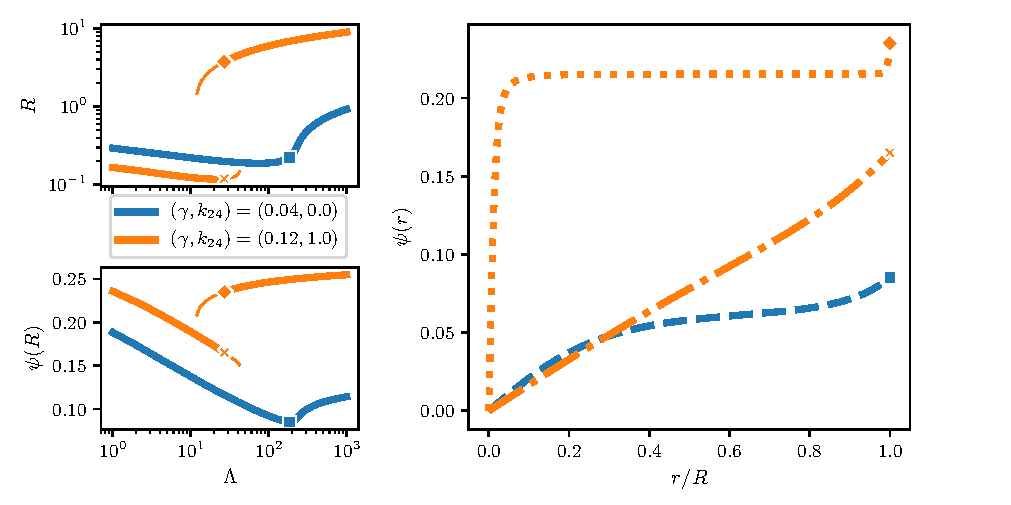
\includegraphics[width=6.74in]{{Figures/_radial-twopair_3.0000e+01_1.0000e+01}.pdf}
    \label{fig:radius_vs_Lambda}}
    \subfloat{
    \label{fig:surf_vs_Lambda}}
    \subfloat{
    \label{fig:psi_vs_r}}
	\caption{Radial structure of a phase-field collagen fibril. \protect\subref{fig:radius_vs_Lambda} Fibril radius, $R$, vs the coupling strength $\Lambda$ between axial and radial structure at constant $\omega=10$. The solid blue line maps the behaviour of $R$ vs $\Lambda$ at surface tension $\gamma=0.04$ and saddle-splay $k_{24}=0$. Similarly, $R$ vs $\Lambda$ for ($\gamma$, $k_{24}$)=(0.12,1) is indicated by both the upper and lower branches of the the solid orange line.  The thin line in the lower branch starting at $\Lambda=27$ indicates a region of meta-stability for a small radius fibril structure. The thin line of the upper branch  which ends at $\Lambda=27$ corresponds to a region of meta-stability for a large radius fibril structure. \protect\subref{fig:surf_vs_Lambda} Surface twist, $\psi(R)$, vs $\Lambda$ for ($\gamma$, $k_{24}$)=(0.04,0) (blue solid line) and ($\gamma$,$k_{24}$)=(0.12,1) (both branches of the orange solid line). Thin lines correspond to meta-stable regions as in \protect\subref{fig:radius_vs_Lambda}. \protect\subref{fig:psi_vs_r} Local, average orientation of tropocollagen molecules within a collagen fibril, $\psi(r)$, vs radial distance from the fibril centre $r$, rescaled by the fibril radius $R$. The dashed blue line in Figure \ref{fig:psi_vs_r} illustrates the inner twist $\psi(r)$ at ($\gamma$, $k_{24}$)=(0.04,0) and $\Lambda=184$. This corresponds to the turning point in \protect\subref{fig:surf_vs_Lambda} where surface twist $\psi(R)$ begins to increase with $\Lambda$. The dotted orange line corresponds to $\psi(r)$ for ($\gamma$, $k_{24}$)=(0.12,1) in the large radius branch of \protect\subref{fig:radius_vs_Lambda} when both structures have equal energy ($\Lambda=27$). We refer to this structure $\psi(r)$ structure as the frustrated twist fibril phase. The dot-dashed orange line corresponds to $\psi(r)$ for the small radius branch at coexistence, $\Lambda=27$. We refer to this $\psi(r)$ structure as the ``linear" twist fibril phase.}\label{fig:obs_radial_vs_Lambda}
\end{figure*}

In Figure \ref{fig:obs_radial_vs_Lambda}, we have selected two pairs of dimensionless surface tension and saddle-splay parameters ($\gamma$, $k_{24}$)=(0.04,0) and ($\gamma$, $k_{24}$)=(0.12,1), to illustrate the two qualitatively different behaviours of our observable parameters as Lambda increases, at a constant $\omega=10$. A more systematic examination of our model behaviour as $k_{24}$, $\gamma$, and $\omega$ are varied is shown in Supplementary Figure \ref{supfig:Lambda_omega}.

In Figure \ref{fig:radius_vs_Lambda}, the dimensionless radius, $R$, of the fibril initially decreases as $\Lambda$ is increased for both sets of ($\gamma$, $k_{24}$) values. At ($\gamma$, $k_{24}$)=(0.04,0.0), there is a smooth transition from decreasing $R$ with Lambda to monotonically increasing $R$ at $\Lambda=74$. In Figure \ref{fig:surf_vs_Lambda}, a similar initial decrease in surface twist occurs as $\Lambda$ is increased. However, the transition to increasing $\psi(R)$ occurs at $\Lambda=184$, and so for the region $74<\Lambda<184$, there is a decrease in $\psi(R)$ while $R$ is increasing.

At ($\gamma$, $k_{24}$)=(0.12,1.0), a discontinuity in both $R$ and $\psi(R)$ occurs at $\Lambda_c=27$, as can be seen in Figure \ref{fig:radius_vs_Lambda} and Figure \ref{fig:surf_vs_Lambda}, respectively. The overlapping of the lower and upper branches of $R$ and $\psi(R)$ indicate that two energy minima exist within the domain $11\leq\Lambda\leq43$ (see Figure \ref{fig:E_vs_Lambda} below). Thin lines illustrate the regions of meta-stability in both the small radius ($\Lambda<\Lambda_c$) and large radius ($\Lambda>\Lambda_c$) fibril structures. This meta-stability is indicative of a discontinuous phase transition between the small and large fibril structures. From Figure \ref{fig:radius_vs_Lambda} and Figure \ref{fig:surf_vs_Lambda}, we see that at the coexistence (i.e. equal energy) point $\Lambda_c=27$, the radius and twist of the small (large) fibril structure are $R=0.1188$ and $\psi(R)=0.1652$ ($R=3.766$ and $\psi(R)=0.2352$), respectively. When there is a discontinuous transition in our observable parameters (as is the case for ($\gamma$, $k_{24}$)=(0.12,1) in Figure \ref{fig:obs_radial_vs_Lambda} above), we refer to fibrils which are in the lower branch ($\Lambda<\Lambda_c$ for equilibrium fibrils) as being part of the ``linear" twist fibril phase. Similarly, we will refer to fibrils in the upper branch as being members of the frustrated twist fibril phase. 

In Figure \ref{fig:psi_vs_r}, we show average local twisting of tropocollagen molecules within the fibril, $\psi(r)$, as the radial distance $r$ from the centre of the fibril increases. The three curves in Figure \ref{fig:psi_vs_r} exemplify the inner structure of fibrils in three different cases. The dashed, blue line in Figure \ref{fig:psi_vs_r} shows the structure of a fibril at $\Lambda=184$ with ($\gamma$, $k_{24}$)=(0.04,0) (i.e. when no discontinuous transition in $R$ and $\psi(R)$ is present for variations in $\Lambda$). We have chosen $\Lambda=184$ as it is near where $R$ and $\psi(R)$ begin increasing with $\Lambda$, and shows intermediate behaviour between a linear twist fibril and a frustrated twist fibril. In Supplementary Figure \ref{supfig:continuouspsi}, we show that increasing values of $\Lambda$ (and so stronger coupling between the d-band modulation and the twisting of the molecules) cause $\psi(r)$ to flatten out at intermediate distances between the fibril centre and the fibril surface, consistent with the dashed blue curve in Figure \ref{fig:psi_vs_r}. Conversely, when ($\gamma$, $k_{24}$)=(0.12,1), we see a distinct transition in the structure of $\psi(r)$ right at coexistence point, $\Lambda_c$. This feature is illustrated in the two orange curves of Figure \ref{fig:psi_vs_r}. The dotted orange line corresponds to the linear twist phase, and the dot-dashed orange line corresponds to the frustrated twist phase, both of which are at $\Lambda_c=27$.

\begin{figure}[t]
    \centering
    \subfloat{
	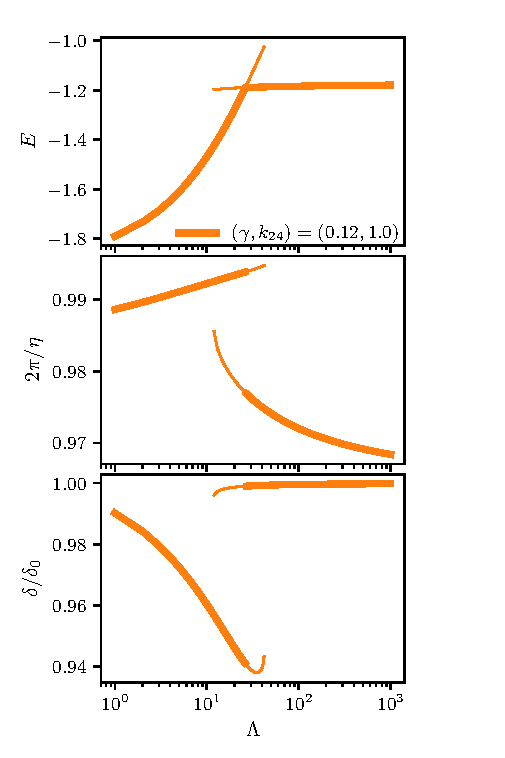
\includegraphics[width=3.37in]{{Figures/_E-eta-delta-twopair_3.0000e+01_1.0000e+01}.pdf}\label{fig:E_vs_Lambda}}
	\subfloat{\label{fig:eta_vs_Lambda}}
	\subfloat{\label{fig:delta_vs_Lambda}}
	\caption{Free energy and axial structure of a phase-field collagen fibril. \protect\subref{fig:E_vs_Lambda} The free energy per unit volume of fibrils, $E$, vs the coupling strength $\Lambda$ between axial and radial structure for two sets of surface tension $\gamma$ and saddle-splay $k_{24}$ parameters at constant $\omega=10$. The blue and orange curves correspond to ($\gamma$, $k_{24}$)=(0.04,0) and ($\gamma$, $k_{24}$)=(0.12,1), respectively. Two free energy minima occur in the region $11\leq\Lambda\leq43$. The thin orange lines which emerge at $\Lambda=27$ indicate meta-stable fibril structures which arise from the presence of a second free energy minimum. \protect\subref{fig:eta_vs_Lambda} The axial period of the d-band (density) modulations, $2\pi/\eta$, vs $\Lambda$. $2\pi/eta=1$ would correspond to a perfect d-band (i.e. with no molecular twist). \protect\subref{fig:delta_vs_Lambda} D-band modulation amplitude, $\delta$, vs $\Lambda$. Any non-zero value of $\delta$ indicates that axial periodicity is present in the fibril.}\label{fig:e_eta_delta_vs_Lambda}
\end{figure}

Figure \ref{fig:e_eta_delta_vs_Lambda} shows the free energy per unit fibril volume, $E$, d-band period, $2\pi/\eta$, and d-band amplitude, $\delta$, that concur with the radial configurations of Figure \ref{fig:obs_radial_vs_Lambda} (at $\omega=10$). The thick orange line in Figure \ref{fig:E_vs_Lambda} is the equilibrium $E$ at ($\gamma$, $k_{24}$)=(0.12,1). The thin orange lines in the region $11\leq\Lambda\leq43$ which branch out at $\Lambda=27$ correspond to the meta-stable energies of the linear twist phase ($\Lambda_c>27$) and the frustrated twist phase ($\Lambda_c<27$). In contrast, $E$ vs $\Lambda$ for ($\gamma$, $k_{24}$)=(0.04,0) (blue line) has no region of meta-stability. For both parameter sets, the energy increases rapidly for small $\Lambda$, and flattens out for large $\Lambda$. Unlike $R$ and $\psi(R)$, $E$ does vary with variations in $\omega$ as can be seen in Supplementary Figure \ref{supfig:LambdaOmegaE}. However, this variation is essentially linear in $\omega$, as expected from eqn \ref{eq:Edw}. In Figure \ref{fig:eta_vs_Lambda} and Figure \ref{fig:delta_vs_Lambda}, we see that the dependence of d-band amplitude and period, $\delta$ and $2\pi/\eta$ also have two distinct regions above and below the critical value $\Lambda_c=27$ for ($\gamma$, $k_{24}$)=(0.12,1), and a single smooth transition for ($\gamma$, $k_{24}$)=(0.04,0).



\subsection{\label{sub:elasticproperties}Elastic properties of the phase field collagen fibril}
%plots of stress, surface twist, local psi(r), delta vs strain, young's modulus vs Lambda for different omega values

%Narrow in on collagen a bit more, by saying "if we have tendon fibrils (low twist, big radius), then what kind of modulus do we have?

%key points:
%i) stress strain curves illustrating non-monotonic, non-linear behaviour for different Lambda values
%ii) Lambda and omega relationship with young's modulus



\section{\label{sec:discussion}Discussion}
\subsection{\label{sub:linear}Linear twist phase}
comparison to descriptive constant pitch phase.
\subsection{\label{sub:nonlinear}Frustrated twist phase}
comparison to descriptive constant twist phase.
\subsection{\label{sub:strain}Compatibility of d-band and molecular twist}
%strain plots with strain cross section.

%can both phases be compatible with d-band? looks like yes, as the strain required on the molecules to allow rope-like twist and d-band is really tiny!

% psi(R) vs d-band to see if d~cos(psi)


\section{\label{sec:conclusion}Conclusion}
\section{\label{sec:references}References}

Because REV\TeX\ uses the \verb+natbib+ package of Patrick Daly, 
the entire repertoire of commands in that package are available for your document;
see the \verb+natbib+ documentation for further details. Please note that
REV\TeX\ requires version 8.31a or later of \verb+natbib+.

\end{document}
%
% ****** End of file apssamp.tex ******
